\documentclass{article}
\usepackage[utf8]{inputenc}
\usepackage[utf8]{inputenc}
\usepackage{graphicx,epstopdf,subfigure,mathtools,mathrsfs} 
\usepackage[normalem]{ulem}
\PassOptionsToPackage{usenames,dvipsnames}{xcolor}
\usepackage[usenames,dvipsnames]{xcolor}
\newcommand{\cmt}[1]{\color{blue}#1\normalcolor}
\newcommand{\norm}[1]{\left\lVert #1 \right\rVert} 
\newcommand{\mat}[1]{\mathbf{#1}}
% notation
\newcommand{\bm}[1]{\mbox{\boldmath $ #1 $}}    % bold math mode
\renewcommand{\vec}[1]{\bm{#1}}                 % vector notation
\def\cddot{% two dots stacked vertically
  \mathbin{\vcenter{\baselineskip.67ex
    \hbox{\onedot}\hbox{\onedot}}%
  }}
  \usepackage{hyperref}
\hypersetup{
    colorlinks=false,
    pdfborder={0 0 0},
}

% Set the margins for 1" around
\setlength{\topmargin}{-0.5in}
\setlength{\oddsidemargin}{0.1in}
\setlength{\evensidemargin}{0.0in}
\setlength{\textwidth}{6.4in}
\setlength{\textheight}{8.9in}

\title{Weak formulation for local slender body theory}
\author{Ondrej Maxian and Aleks Donev}

\begin{document}

\maketitle
\section{Method formulation}
We are interested in modeling inextensible, slender fibers using slender body theory. Thus our task is to solve the PDE
\begin{equation}
\label{eq:fibevcont}
\frac{\partial \bm{X}}{\partial t} -\bm{U}_0(\bm{X})= \bm{M}\left(\bm{f}^{E}+\bm{\lambda}\right),
\end{equation}
where $\bm{M}$ is a mobility operator that comes from slender body theory and $\bm{U}_0$ is a background flow. $\bm{f}^E$ are the bending forces on the fiber, and $\bm{\lambda}=(T\bm{X}_s)_s$ are tensile forces that act as Lagrange multipliers enforcing inextensibility of the fiber. The fibers are assumed to be free, and are therefore subject to the boundary conditions, $\displaystyle \bm{X}_{ss}\left(s=0,L\right)=\bm{X}_{sss}\left(s=0,L\right)=\bm{0}$. 

\subsection{Slender body theory}
In slender body theory, the 3D slender fiber with aspect ratio $\displaystyle{\epsilon = \frac{r(L/2)}{L}}$ is reduced to a one dimensional curve along the fiber centerline via an asymptotic expansion in $\epsilon$. The slender body mobility operator is given by
\begin{equation}
\label{eq:Msbt}
\bm{M}[\bm{f}](s) =\frac{1}{8\pi \mu}\left( \bm{ \Lambda}[\bm{f}](s)+\bm{J}[\bm{f}](s)\right),
\end{equation}
where $\bm{f}$ is the force per length on the fiber. The first term on the right side of Eq.\ \eqref{eq:Msbt} is the local operator $\bm{\Lambda}$ given by
\begin{equation}
\label{eq:localsbt}
\bm{\Lambda}=-\log{(\epsilon^2 e)}(\bm{I}+\bm{X}_s \bm{X}_s) + 2(\bm{I}-\bm{X}_s \bm{X}_s). 
\end{equation}
Notice that, because the fiber is inextensible, $\bm{X}_s$ is assumed to be a unit vector, and $\bm{X}_s \bm{X}_s$ is an outer product. Using the $\mathcal{O}(\log{\epsilon^2})$ term of $\bm{\Lambda}$ in place of $\bm{M}$ is synonymous with the \textit{local drag model}. In addition, note that the definition of $\bm{\Lambda}$ in Eq.\ \eqref{eq:localsbt} gives a slender body theory that is $\mathcal{O}(\epsilon^2)$ accurate for \textit{ellipsoidal fibers}, that is, fibers whose radius is given by $r(s)=2\epsilon \sqrt{s(L-s)}$, where $s\in[0,L]$. For cylindrical fibers, this form of SBT is $\mathcal{O}(1)$ accurate, and a different form of $\bm{\Lambda}$ must be used to give the same asymptotic accuracy. In particular, for a general radius $r(s)=a(s)\epsilon L$, the local term is given by  
\begin{align}
\label{eq:c_t_general}
\bm{\Lambda} =\left(c\left(\frac{2s}{L}-1\right)(\bm{I}+\bm{X}_s\bm{X}_s) +  (\bm{I}-3\bm{X}_s\bm{X}_s)\right)\bm{f}(s)
\end{align}
where
\begin{equation}
c(t) = \log{\left(\frac{2(1-t^2)+2\sqrt{(1-t^2)^2+16\epsilon^2a(t)^2}}{4a(t)^2\epsilon^2}\right)}.
\end{equation}
For a cylindircal fiber $a(t)=1$. This expression is taken from \cite{morifree} and is chosen so that $c(t) < \infty$ at the fiber ends.

For either cylindrical or ellipsoidal fibers, the $\mathcal{O}(1)$ non-local integral operator $\bm{J}$ is given by
\begin{equation}
\label{eq:intsbt}
\bm{J}[f](s) = \int_0^L \left(\frac{\bm{I}+\hat{\bm{R}}(s,s')\hat{\bm{R}}(s,s')}{\norm{\bm{R}(s,s')}}\bm{f}(s') - \frac{\bm{I}+\bm{X}_s(s) \bm{X}_s(s)}{|s-s'|} \bm{f}(s) \right) ds',
\end{equation}
where $\bm{R}(s,s')=\bm{X}(s)-\bm{X}(s')$ and $\hat{\bm{R}}$ is the corresponding unit vector. We will put off study of the non-local integral until a later time. 

\textbf{For the rest of this report, unless otherwise indicated, we set $\bm{M}=\bm{\Lambda}$ in Eq.\ \eqref{eq:localsbt} to compare with the data received from Floren}, which is obtained using a linearly implicit spectral discretization based on Tornberg and Shelley \cite{ts04}.

\input{ForPaperTh.tex}

\subsection{Discrete weak formulation}
\input{DiscrWk.tex}

\subsection{Evolving the tangent vector $\V{X}_s$}

A good choice of normal vectors that has a clear physical meaning is based on the Euler angles $\theta$ and $\phi$ for the unit tangent vector $\V{X}_s$,
\begin{equation}
\V{X}_s(\theta(s,t),\phi(s,t)) = \begin{pmatrix} \cos{\theta} \cos{\phi}\\[2 pt] \sin{\theta} \cos{\phi} \\[2 pt] \sin{\phi} \end{pmatrix}.
\end{equation}
The choice of normal vectors that is always orthonormal to $\V{X}_s$ on the unit sphere is
\begin{equation}
\label{eq:nangles}
\V{n}_1 =  \begin{pmatrix} -\sin{\theta}\\[2 pt] \cos{\theta}\\[2 pt]0 \end{pmatrix} \qquad \V{n}_2 =  \begin{pmatrix} -\cos{\theta} \sin{\phi}\\[2 pt] -\sin{\theta} \sin{\phi} \\[2 pt] \cos{\phi} \end{pmatrix}. 
\end{equation}
The position of the fiber $\V{X}$ can be recovered by 
\begin{equation}
\label{eq:XfromXs}
\V{X}(s)= \V{X}(0)+\int_0^s \V{X}_s(\theta(s),\phi(s)) \, ds. 
\end{equation}

By the right-handedness of the coordinate system
\begin{equation}
\label{eq:Xsupdate}
\V{X}_{st} = g_1(s)\V{n}_1 + g_2(s) \V{n}_2 = \left(g_1(s)\V{n_2}-g_2(s)\V{n}_1\right) \times \V{X}_s:=\V{\Omega}\left(\V{X}_s, \V{\alpha}\right) \times \V{X}_s. 
\end{equation}
Therefore, $\V{\Omega}\left(\V{X}_s, \V{\alpha}\right)=g_1(s)\V{n_2}-g_2(s)\V{n}_1$ can be viewed as a rotational velocity for $\V{X}_s$ on the unit sphere. The notation here indicates that $\V{\alpha}$ determines $g_1$ and $g_2$ and therefore $\V{\Omega}$. We will use this to update the configuration in our temporal integration schemes by rotating the tangent vector $\V{X}_s$ and then computing $\V{X}$ using \eqref{eq:XfromXs}; this strictly enforces inextensibility.

This theory is of course predicated on the smoothness of $\V{n}_1(s)$ and $\V{n}_2(s)$. In Eq.\ \eqref{eq:nangles}, it is clear that this only holds if $\theta$ is single-valued at $\phi=\pi/2$. Otherwise the signs of $\V{n}_1$ and $\V{n}_2$ can oscillate. We therefore set $\theta \left(\phi=\pm \pi/2\right)=0$ (numerically: \texttt{theta(abs((abs(phi)-pi/2)) < 1e-12) =0}). 

\subsection{Thermal Fluctuations}

This section was written by Aleks.

Let us summarize the equations of motion in the $L_2$ weak form, which appears to be most suitable to stochastic evolution on a space of inextensible worm-like chains. We add here Brownian noise following \cite{FluctuatingFibers_Saintillan_PNAS,FluctuatingFibers_Saintillan_PF}. Although this and all other prior work we know of was not careful about subtleties of multiplicative noise and infinite-dimensional Fokker-Planck equations, I believe ``the physicists" have the right form for the noise covariance and are (most likely) only missing some stochastic drift terms. In this section, we focus on a single fiber and we will ignore the translational motion of the fiber, which means we will set $\V{U}= {\partial\V{X}}/{\partial t}(s=0,t) = \V{0}$ as this is the easy part.

In order to avoid constraints, we will write here the evolution for the unit tangent vector along the fiber $\V{X}_s(\theta(s,t),\phi(s,t)) = \left( \cos{\theta} \cos{\phi},\, \sin{\theta} \cos{\phi},\,  \sin{\phi} \right)$ instead of $\V{X}$, but the inextensibility constraint will be implicit in the dynamical equations which arise from enforcing it with a tension Lagrange multiplier. Recall that we can complete $\V{X}_s$ to an orthonormal triad with the two orthogonal vectors $\V{n}_1(s)$ and $\V{n}_2(s)$ given in \eqref{eq:nangles}. While one could use the spherical angles $\theta(s,t)$ and $\phi(s,t)$ to describe the configuration this poses a problem at special points (e.g., the North pole) and is not very natural, so we instead think of $\V{X}_s(s,t)$ as being a curve on the unit sphere $S_2$ that evolves in time. The actual configuration $\V{X}(s,t)$, which enters in the equations also, is computed by integration of $\V{X}_s(s,t)$ using \eqref{eq:XfromXs}.

Recall that the process begins by choosing a set of basis functions $\phi_k(s)$ for $L_2:[0,s]$, which in the discrete formulation we take to be Chebyshev polynomials but this is not required. The dynamics of the fiber tangent vector is given by
\begin{equation}
\label{eq:Xsupdate_fluct}
\V{X}_{st} = \left( \M{K} \V{\alpha}\right)(s) = \V{\Omega}(s,t) \times \V{X}_s, 
\end{equation}
where
\begin{equation}
\label{eq:Omega_fluct}
\V{\Omega}(s,t) = \V{\Omega}\left(\theta(s,t),\phi(s,t), \V{\alpha}(t)\right) = 
	\sum_k \left[ \alpha_{1k}(t) \phi_k(s) \V{n_2}(s) - \alpha_{2k}(t) \phi_k(s) \V{n}_1(s) + \dots \right],
\end{equation}
where the dots indicate missing stochastic drift terms that we don't yet have any idea about except that they should be proportional to $k_B T$.

The direction of motion $\bm{\alpha}(t)=(\alpha_{1k}(t),\alpha_{2k}(t))$ (here $k$ is an index counting the basis functions) in the tangent to the manifold of inextensible fibers, as well as the constraint force density $\V{\lambda}(s,t)$, are computed by solving the saddle-point system
\begin{equation}
\label{eq:saddleL2_fluct}
\begin{pmatrix}
-\bm{M} & \bm{K}\\[4 pt]
\bm{K}^* & \bm{0}
\end{pmatrix}
\begin{pmatrix} 
\bm{\lambda}\\[4 pt]
\bm{\alpha}\\[4 pt]
\end{pmatrix} =  \begin{pmatrix} 
\bm{M}\bm{L}\bm{X} + \sqrt{2 k_B T} \bm{M}^{\frac{1}{2}} \V{\zeta} \\[4 pt]
\bm{0}\end{pmatrix},
\end{equation}
where $\V{\zeta}(s,t)$ is white noise in space and time. The specific form of the basis functions enters in the operator $\bm{K}$ defined via \eqref{eq:Xsupdate_fluct}, and its $L_2$ adjoint $\bm{K}^*$. Note that for the local drag model $\bm{M}=\bm{\Lambda}/(8\pi\mu)$, an explicit formula for the Brownian force density can be written (personal communication with David Saintillan):
\begin{equation}
\V{f}^B(s,t) = \sqrt{\frac{2 k_B T}{8\pi\mu}} \left(\bm{\Lambda}^{\frac{1}{2}} \V{\zeta}\right)(s,t) =  
	\sqrt{\frac{2 k_B T}{8\pi\mu}} \left( c_1(s) \M{I} + c_2(s) \V{X}_s \V{X}_s \right) \V{\zeta}(s,t),
\end{equation}
where the form of $c_1(s)$ and $c_2(s)$ can be computed by computing the covariance of $\V{f}^B$ and comparing it against \eqref{eq:c_t_general}. But this form should not be required in the formulation of the algorithm, which should also work even when the mobility includes non-local parts (which should be symmetric positive-definite, though this is not obvious just by looking at \eqref{eq:intsbt}).

Recall that $\bm{L}\V{X}=-E \V{X}_{ssss}$, taking into account the boundary conditions $\V{X}_{ss}=\V{X}_{sss}=0$ at both free ends. It is not clear how to handle the BCs in the context of fluctuating fibers. Should we put BCs somehow in the set of basis functions or should we enforce them as linear constraints on $\V{\alpha}$ as we (sort of) do in the numerical method? My feeling is that probably to get a working \emph{discrete} stochastic formulation in the end we will need to switch to a Galerkin formulation instead of the collocation approach, that is, we would want to replace \eqref{eq:veleq} with its Galerkin projection onto the space spanned by the basis functions. In this case we would enforce the BCs in the Galerkin formulation directly when integrating by parts, which imposes them weakly and not strictly, as seems the right thing to do. It is not clear, however, whether we also need to switch to Galerkin at the semi-formal level of the continuum $L_s$ formulation as well.

What we want from the equilibrium stochastic dynamics is that it be time-reversible with respect to a specific ``worm-like chain" invariant measure. This invariant measure for the tangent vector $\V{X}_s(s)$ is formed by the set of Brownian motions on $[0,L]$ on the unit $S_2$ sphere, where the diffusion coefficient of the Brownian motion is proportional to $k_B T / E$ (note that this means we cannot set $E=0$ and still make sense of this measure). This is more or less all we know, and now our goal is to figure out what to put in for the dots in \eqref{eq:Omega_fluct} to make this be so. The expectation is (but this should also be studied) is that if there is an additional conservative force density $\V{f}^{(c)}=-\delta{E^{(c)}}/\delta{\V{X}}$ other than bending, the dynamics would be time-reversible with respect to the same measure but weighted by the Boltzmann factor $\exp\left(-E^{(c)}\left[\V{X}\right]/\left(k_B T\right)\right)$.

One approach would be to represent Brownian motion on the unit $S_2$ sphere in some basis (say KL expansion), then truncate to get a smooth $\V{X}_s(s)$, and work with this as a function. Or maybe everything should be discretized to turn into a finite-dimensional Langevin equation (but observe this equation is very complicated in the end). These are still wide open questions that require some thought and discussion with Eric and Miranda.



\newpage
\section{Results}
In this section, we compare the output of our algorithm directly with that of Floren for a fiber with initial tangent vector
\begin{equation}
\label{eq:Xst0}
\bm{X}_s(s,t=0) = \frac{1}{\sqrt{2}}\begin{pmatrix} \cos{\left(s^3 (s-L)^3\right)}\\[2 pt] \sin{\left(s^3(s-L)^3\right)}\\[2 pt] 1 \end{pmatrix}. 
\end{equation}
This choice of tangent vector satisfies the boundary conditions $\displaystyle \bm{X}_{ss}\left(s=0,L\right)=\bm{X}_{sss}\left(s=0,L\right)=\bm{0}$ and the inextensibility constraint. Because there is no analytical solution for its configuration, we integrate Eq.\ \eqref{eq:Xst0} forward in $s$ with $\bm{X}(s=0,t=0)=\bm{0}$ to arrive at a configuration of the form $(x(s),y(s),s/\sqrt{2})$. The 2D projection of the fiber (and therefore the form of the functions $x(s)$ and $y(s)$) is shown in Fig.\ \ref{fig:3Dfibt0} as a blue curve. We also show in Fig.\ \ref{fig:3Dfibt0} the fiber configuration at $t=0.01$ for $N=8$ for both our code and Floren's code ($\tilde{N}=12$ - Floren uses a type 2 grid, so all of his data is marked with a tilde). Note the differences at the boundaries; we will establish which is more accurate in subsequent sections. 

In general, we will use an $L^2$ function norm to compute the differences between configurations throughout this section. Given two configurations $\bm{X}$ and $\bm{Y}$, the $L^2$ norm of their difference is defined as
\begin{equation}
\label{eq:Errort}
E[\bm{X},\bm{Y}](t) = \left(\int_0^L \norm{\bm{X}(t)-\bm{Y}(t)}^2 \, ds\right)^{1/2} = \left( \sum_{i=1}^{1000} \norm{\bm{X}(s_i,t)-\bm{Y}(s_i,t)}^2 \, w_i  \right)^{1/2}. 
\end{equation}
The final term denotes the fact that we upsample each configuration to a common type 2 grid of $1000$ points. 

\begin{figure}
\centering 
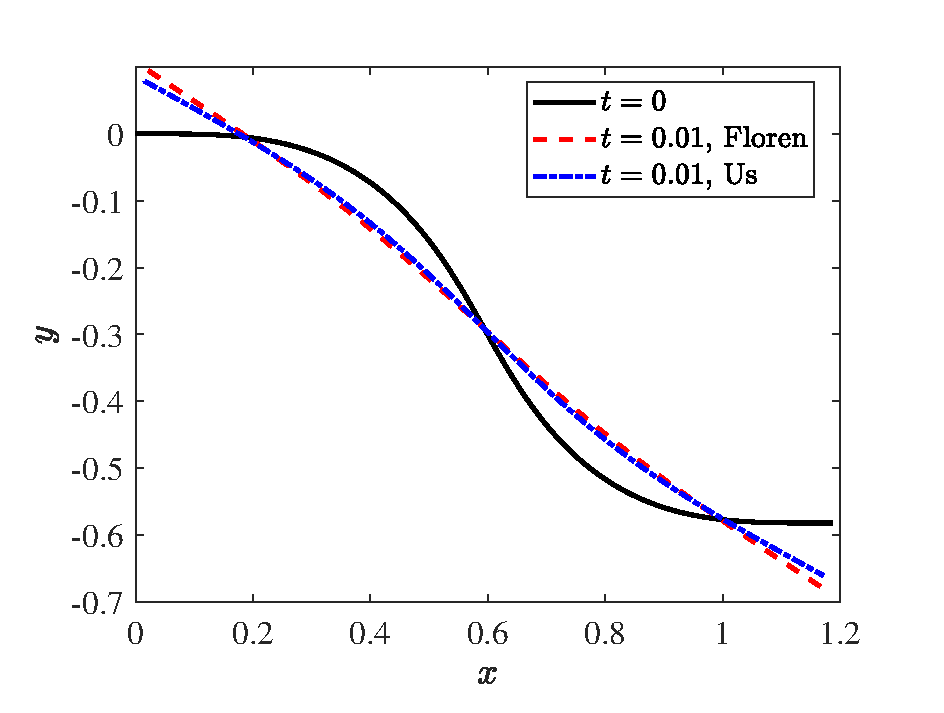
\includegraphics[width=70mm]{FiberInitial.eps}
\caption{Fiber configuration for code comparison (2D projection). The black line shows the initial configuration at $t=0$. The initial $z$ coordinate is simply $z(s)=s/\sqrt{2}$. The final position of the fiber for $N=8, \tilde{N}=12$ points is shown as a dashed red line (for Floren's data) and a dashed/dotted blue line (for our data). Details: Floren's data has $\tilde{N}=12$, $\Delta t =10^{-6}$, our data has $N=8$, $\Delta t=10^{-4}$ (forward Euler update).}
\label{fig:3Dfibt0}
\end{figure}

\subsection{Convergence}
\label{sec:conv}

\subsubsection{Fiber tension at $t=0$}
We compare the values of $\bm{\lambda}$ with $(T\bm{X}_s)_s$ at $t=0$. The latter quantity is obtained by mutiplying the analytically computed (from Eq.\ \eqref{eq:Xst0}) $\bm{X}_s$ by Floren's provided values of tension $T(t=0)$ at each point, and then applying the spectral differentiation matrix. We measure the error of each against the ``exact solution'' of Floren's tensile force for $\tilde{N}=24$. Fig.\ \ref{fig:tension} shows that $\bm{\lambda}$ is indeed converging to $(T\bm{X}_s)_s$. Indeed, the $L^2$ error in $\bm{\lambda}$ for $N=8$ is 2.81, whereas for $N=20$ the $L^2$ error in $\bm{\lambda}$ is $8.3 \times 10^{-3}$. 
\begin{figure}
\centering
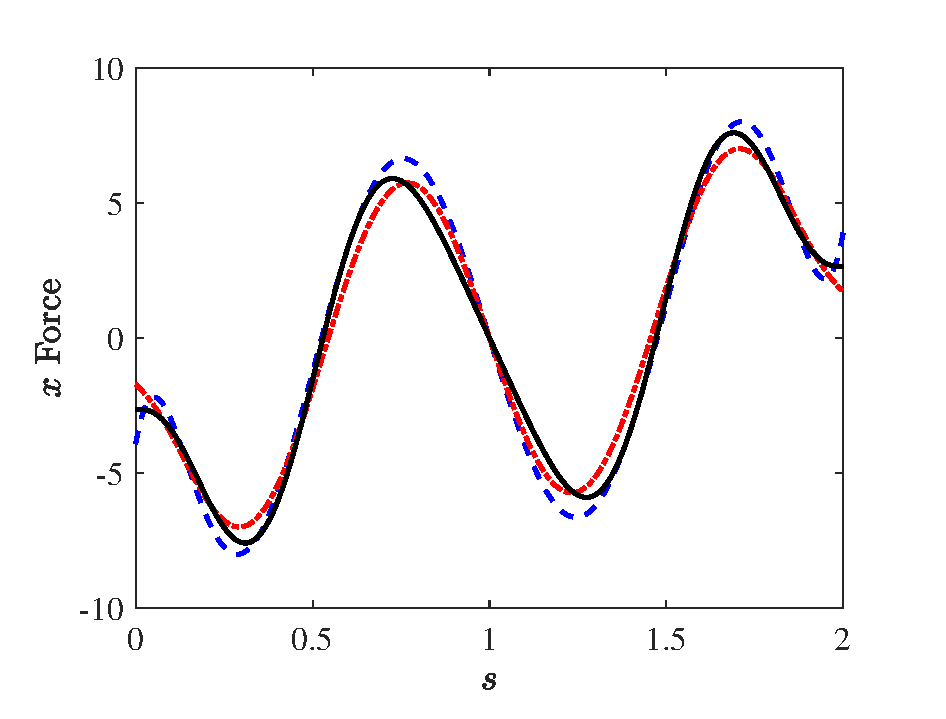
\includegraphics[width=50mm]{TensionX.eps}
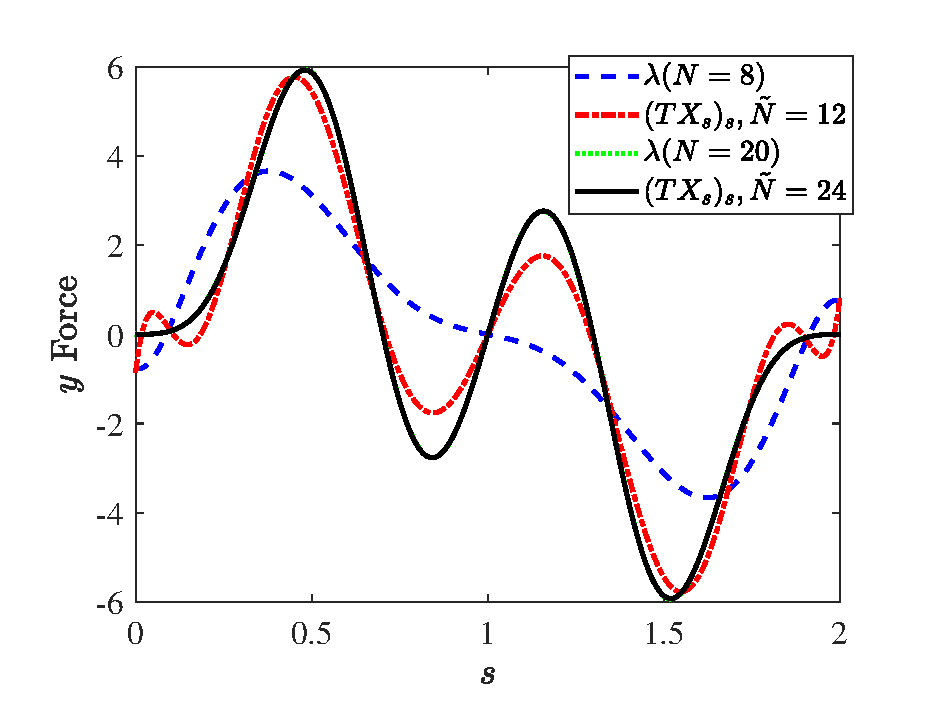
\includegraphics[width=50mm]{TensionY.eps}
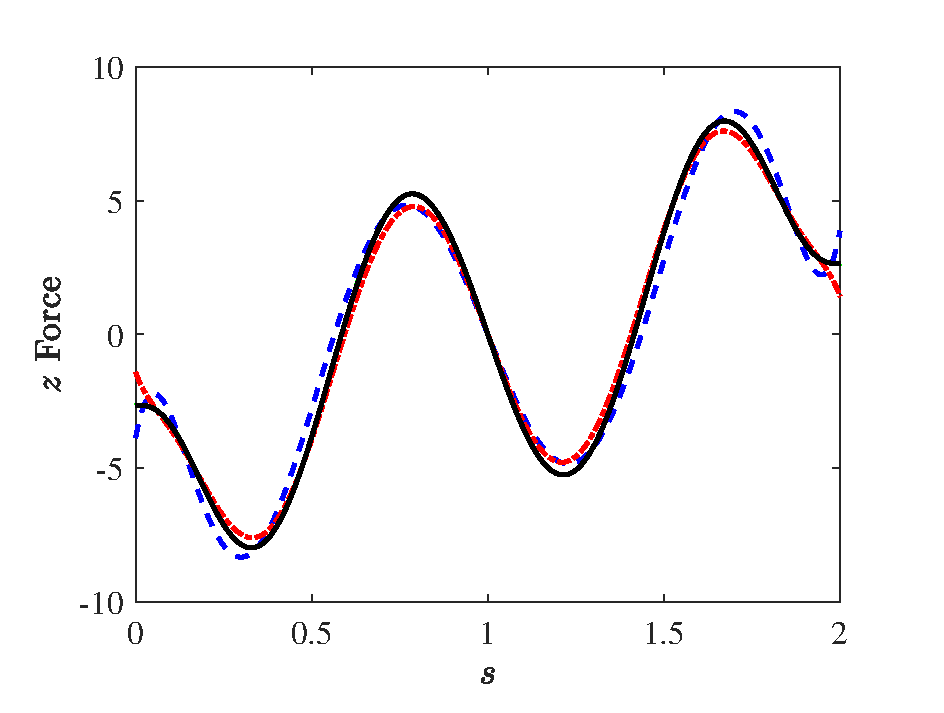
\includegraphics[width=50mm]{TensionZ.eps}
\caption{Measuring the convergence of $\bm{\lambda}$ against $(T\bm{X}_s)_s$. Each direction in the force $(x,y,z)$ is a column from left to right. The dashed blue line shows $\bm{\lambda}$ for $N=8$, which has an $L^2$ error of 2.81. For comparison, Floren's tensile force for $\tilde{N}=12$ is shown as a dashed-dotted red line. It has an $L^2$ error of 1.22. $\bm{\lambda}$ for $N=20$ is shown as a dotted green line, it has $L^2$ error $8.3 \times 10^{-3}$ and is completely indistinguishable from the ``exact'' solution of Floren for $\tilde{N}=24$. }
\label{fig:tension}
\end{figure}

\subsection{Spatial error}
\label{sec:space}
We received 2 simulations from Floren: one with $\tilde{N}=12$ points and one with $\tilde{N}=24$. In this section, we compare the results from the algorithms for both $N=8$ and $N=20$. In order to isolate the \textit{spatial} error, we compare our solution with a strong stability preserving third order Runge Kutta (SSP RK3) time integrator to the solution Floren sent with the lowest timestep. The SSP RK3 solutions are accurate to 10 or more digits, as verified by refining the timestep by a factor of 2 and comparing solutions (for $N=8$, $\Delta t =10^{-6}$, for $N=20$, $\Delta t =10^{-7}$). The ``exact'' solution is defined to be the one Floren sent with $\tilde{N}=24$ and smallest timestep $\Delta t=10^{-6}$. 

Fig.\ \ref{fig:L2} shows the $L^2$ errors of 3 simulations: both ours and Floren's when $N=8, \tilde{N}=12$, and ours when $N=20$. Our algorithm gives 3 digits of \textit{absolute} accuracy in the fiber position for $N=8$ and 4 digits for $N=20$. 

Fig.\ \ref{fig:poser12} gives the absolute error at $t=0.01$ as a function of the arclength position along the fiber for $N=8, 20$ for both Floren's and our simulation. We observe about 3 digits of absolute accuracy for $N=8$ and 4 digits for $N=20$. In general, the relative accuracy is 10 times the absolute accuracy (i.e. 10 times worse), since the points move approximately $\mathcal{O}(0.1)$ throughout the simulation. 

Note also that the absolute accuracy of Floren's solution for $\tilde{N}=12$ is 1-2 digits. This translates to a relative accuracy of 0-1 digit. That is, there is an error of 10-100\% in the motion of the points (especially near to the boundaries). \textbf{Thus the spatial error for our discretization is $10^{-3}$ for $N=8$ points, but for Floren's it is $10^{-2}$, or even larger near the boundary. Thus, at least for this spatial discretization, our algorithm is more accurate. }


\begin{figure}
\centering 
\subfigure[$L^2$ norm]{
\label{fig:L2}
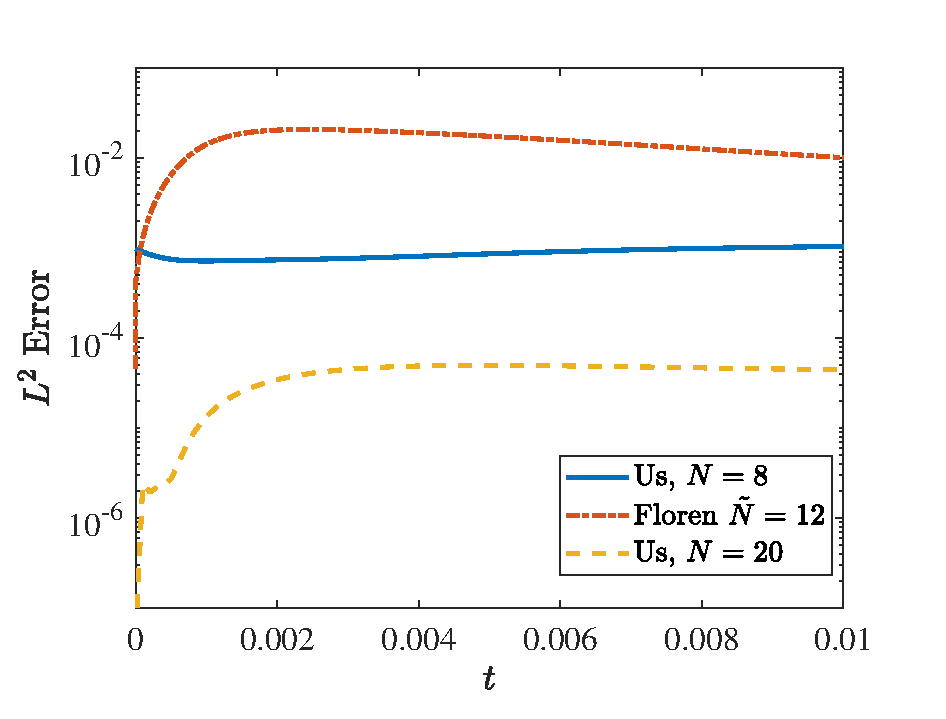
\includegraphics[width=70mm]{SimonsL2Compare.eps}}
\subfigure[Error by position]{
\label{fig:poser12}
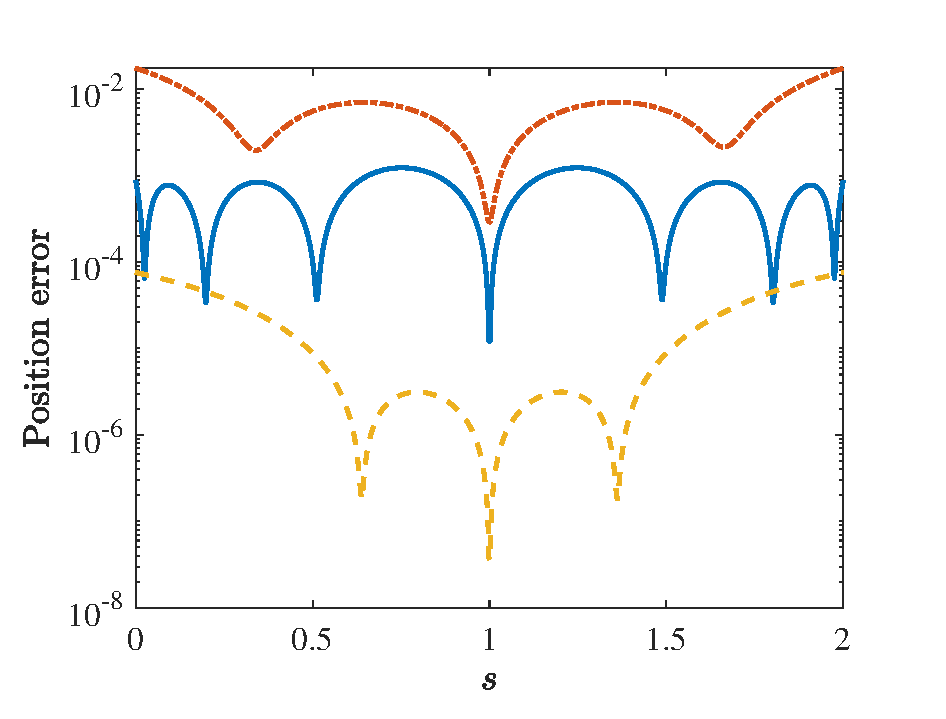
\includegraphics[width=70mm]{ErrorbyPosition.eps}}
\caption{Errors from 3D fiber simulation. (a) $L^2$ norm over time for $N=8$ (solid blue), $N=20$ (dashed yellow). The norm is defined in Eq.\ \eqref{eq:Errort}. The $L^2$ error in Floren's data for $\tilde{N}=12$ is shown as a dashed-dotted red line. (b) The absolute error in the positions along the fiber (at $t=0.01$) for $N=8$, $N=20$ (same color scheme as (a)). The spatial errors are isolated by using an SSP RK3 scheme for our method and using the lowest timestep provided for Floren's method.} 
\end{figure}

\subsubsection{Inextensibility}
\label{sec:inext}
We consider how inextensible the fiber truly is for $t > 0$. In \cite{ts04}, a penalty parameter $\beta$ is added to the line tension equation to preserve inextensibility. In this section, we compare this formulation to our formulation, where the inextensibility is constrained by the allowed fiber motion, Eq.\ \eqref{eq:du}. 

To measure the inextensibility error, we take the fiber positions $\bm{X}$, upsample them to a fine grid, apply the spectral differentiation matrix on the fine grid to compute $\bm{X}_s$, and then measure the maximum difference of its norm from 1 along the fiber at every timestep. Fig.\ \ref{fig:inext} shows the results for simulations with negligible temporal error. While Floren's code with the penalty parameter (solid lines) generally performs better, we are still able to enforce inextensibility to 2  digits for $N=8$ and 6 digits for $N=20$.

\begin{figure}
\centering
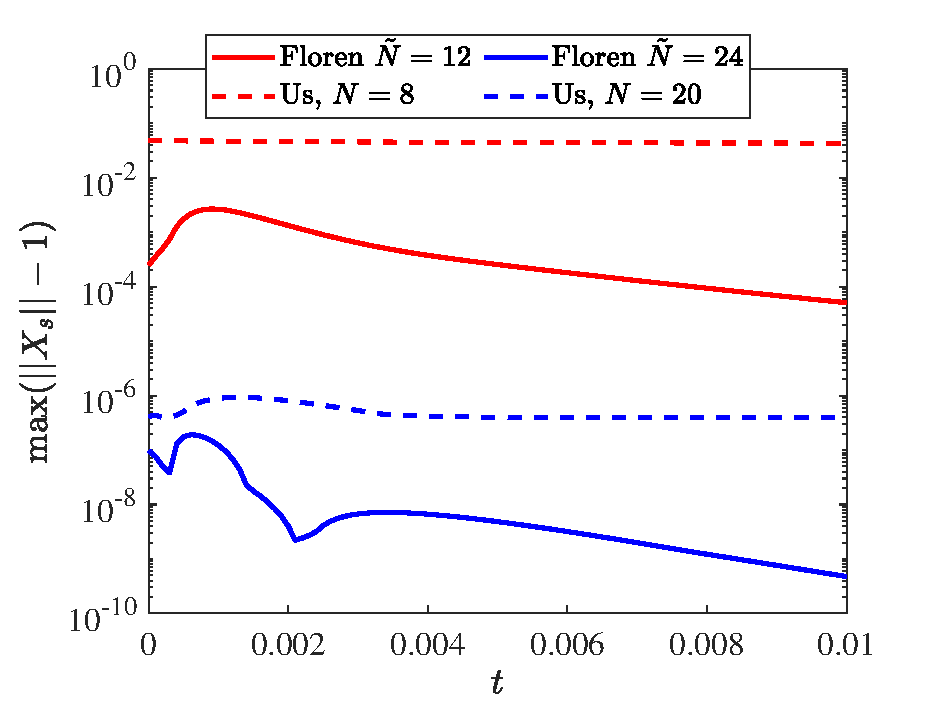
\includegraphics[width=70mm]{Inextensibility.eps}
\caption{Error in enforcing the inextensibility constraint, $\textrm{max}\left|\norm{\bm{X}_s}-1\right|$ for $N=8$, $\tilde{N}=12$ (red lines) and $N=20$, $\tilde{N}=24$ (blue lines). Solid lines show the results from Floren's code with the penalty parameter, while dashed lines show the results for our algorithm with constrained motion. }
\label{fig:inext}
\end{figure}

\subsubsection{Boundary conditions}
One of the features of our method is that boundary conditions are enforced in a weak sense with rectangular matrices (as opposed to a strong sense with square matrices). To verify this, we consider the fiber configuration $\bm{X}$ at time $t$. We perform differentiation on the type 1 grid and upsample the result to a type 2 grid with 1000 points (this is numerically preferable to upsampling and then differentiating). We consider the norms $\norm{\bm{X}_{ss}(s=0)}$ and $\norm{\bm{X}_{sss}(s=0)}$ of the upsampled derivative (these quantities are the same at $s=L$ by symmetry and should both be zero). 

Fig.\ \ref{fig:BCs} shows the error in the boundary conditions as a function of time for $N=8, 12, 16$ and $20$. As in Section \ref{sec:inext}, the configurations are generated using RK3 temporal integration with $\Delta t =10^{-6}$ to isolate the spatial error. For both $\bm{X}_{ss}$ and $\bm{X}_{sss}$, we observe spectral convergence. 

\begin{figure}
\centering 
\subfigure[$\norm{\bm{X}_{ss}(s=0)}$]{
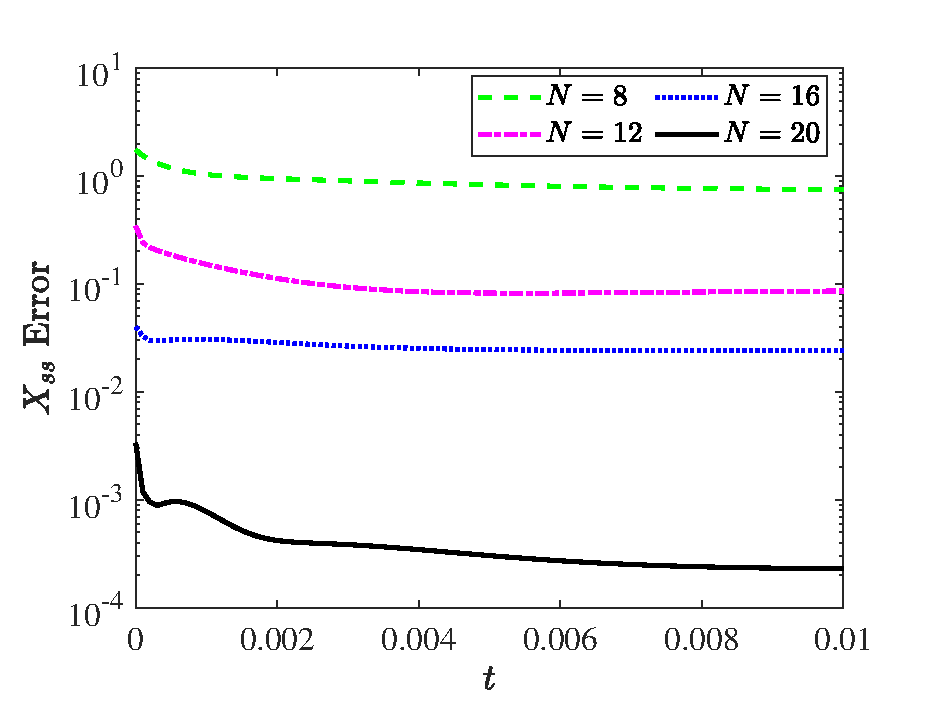
\includegraphics[width=70mm]{BCErrorXss.eps}}
\subfigure[$\norm{\bm{X}_{sss}(s=0)}$]{
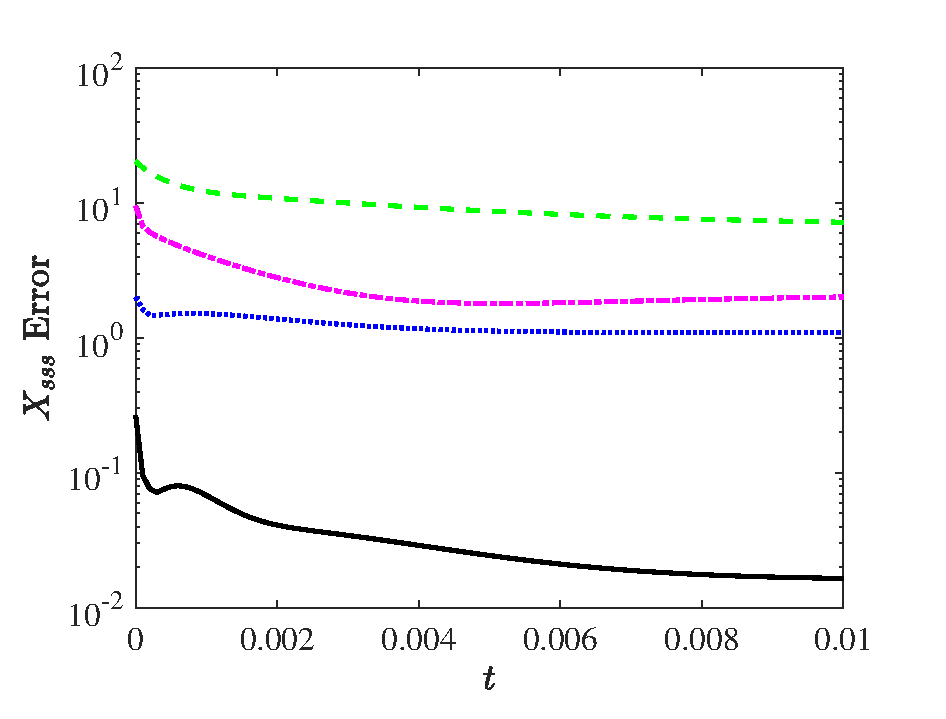
\includegraphics[width=70mm]{BCErrorXsss.eps}}
\caption{Spectral convergence of boundary conditions (a) $\norm{\bm{X}_{ss}(s=0)}_2$, (b) $\norm{\bm{X}_{sss}(s=0)}_2$, both of which should be 0. Shown are solutions for $N=8$ (dashed green), $N=12$ (dashed-dotted pink), $N=16$ (dotted blue), and $N=20$ (solid black), all simulated with RK3 so that the temporal integration is accurate to 10 digits. Values at the boundaries are obtained by differentiation on the $N$ grid, then upsampling to a type 2 grid (that includes the endpoints). }
\label{fig:BCs} 
\end{figure}


\subsection{Temporal error}
\label{sec:temp}
Having studied the spatial error in detail, we next study the temporal error and the requisite timestep to achieve a certain accuracy across both algorithms. 
\subsubsection{Floren's data}
We begin with an analysis of Floren's data. Again, the ``exact'' solution is Floren's fiber evolution for $\tilde{N}=24$, $\Delta t =10^{-6}$ (the finest spatial and temporal discretization provided). Fig.\ \ref{fig:FN12} shows the $L^2$ errors for $\tilde{N}=12$ and a variety of timesteps for Floren's algorithm. We observe the $L^2$ errors in Floren's algorithm for $\tilde{N}=12$ are more or less saturated by the spatial error. Even for a timestep as small as $10^{-6}$, there is still an $L^2$ error of $\mathcal{O}(10^{-2})$. 

Given the large spatial error, it remains to be seen what timestep Floren has to use to get a temporal error less than or equal to the spatial error for $\tilde{N}=12$. As shown in Fig.\ \ref{fig:FN12temp}, a timestep of $\Delta t =10^{-3}$ gives an $L^2$ difference of $\approx 0.015$ from the evolution when $\Delta t =10^{-6}$. Given that the spatial error is $\approx 0.01$, we conclude that \textbf{Floren can use a $\Delta t =10^{-3}$ for $\tilde{N}=12$ and get a temporal error less than or equal to the spatial error}. 

\begin{figure}
\centering 
\subfigure[``Error'' wrt $\tilde{N}=24$]{
\label{fig:FN12}
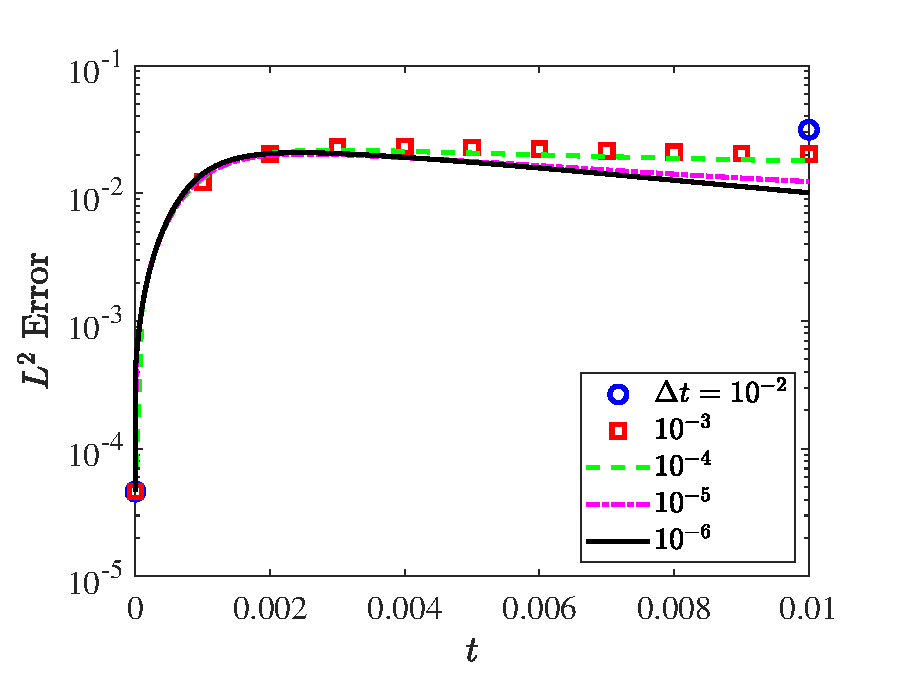
\includegraphics[width=70mm]{Local/FlorenTemporalN12.eps}}
\subfigure[``Error'' wrt $\tilde{N}=12$]{
\label{fig:FN12temp}
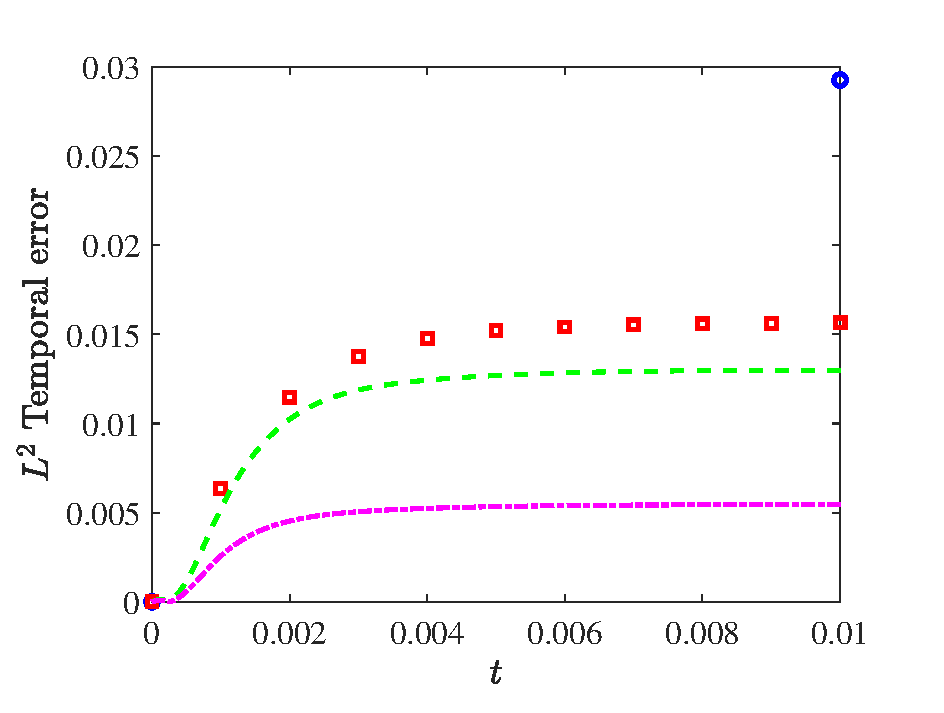
\includegraphics[width=70mm]{Local/FlorenN12Temporal.eps}}
\caption{(a) $L^2$ errors over time when comparing to Floren's ``exact'' solution with $\tilde{N}=24$, $\Delta t=10^{-6}$ to his solutions when $\tilde{N}=12$. (b) $L^2$ \textit{temporal} errors in Floren's algorithm for $\tilde{N}=12$ using $\tilde{N}=12$ $\Delta t = 10^{-6}$ as the ``exact'' solution. Timesteps are color coded as blue circles ($10^{-2}$), red squares ($10^{-3}$), dashed green lines ($10^{-4}$), dashed-dotted pink lines ($10^{-5}$), and solid black lines ($10^{-6}$). } 
\label{fig:Flortemp}
\end{figure}

\subsubsection{Accuracy of temporal integration for fixed spatial discretization}
\label{sec:rk3fe}
We next focus on our algorithm with a fixed spatial discretization. For simplicity and ease of running multiple simulations, we choose $N=8$. We first check the order of accuracy of the SSP RK3 scheme
\begin{gather}
\bm{X}^{n+1} = \bm{X}^n + \Delta t \left(\frac{1}{6}\bm{k}_1 + \frac{1}{6}\bm{k}_2+\frac{2}{3}\bm{k}_3\right)\\[4 pt]
\bm{k}_1 = \bm{u}\left(\bm{X}^n\right) \qquad \bm{k}_2 = \bm{u}\left(\bm{X}^n + \Delta t \bm{k}_1\right) \qquad \bm{k}_3 = \bm{u}\left(\bm{X}^n + \frac{\Delta t}{4} \bm{k}_1 + \frac{\Delta t}{4} \bm{k}_2\right).
\end{gather}
Importantly, for this test we will use successive refinements to measure convergence (rather than comparing to Floren's results). As shown in Fig.\ \ref{fig:RK3N8}, SSP RK3 is a third order accurate scheme, as the errors scale as $\Delta t^3$. Importantly, the temporal error for $\Delta t = 10^{-4}$ using RK3 is $10^{-5}$, which is 2 orders of magnitude less than the spatial error of $10^{-3}$ (see Fig.\ \ref{fig:L2}). Furthermore (this data is not shown on the plot), using $\Delta t = 2 \times 10^{-4}$ gives a maximum $L^2$ error of $9 \times 10^{-5}$ and $\Delta t = 4 \times 10^{-4}$ gives a maximum $L^2$ error of $2 \times 10^{-2}$ in RK3. 

Next, we take the solution from SSP RK3 with $\Delta t =10^{-6}$ and treat this (which has converged to 12 digits) as an exact solution for $N=8$. We seek the error from forward Euler. The timestep $\Delta t =10^{-3}$ is unstable. As shown in Fig.\ \ref{fig:FEN8}, using a timestep half of this unstable $\Delta t$ yields a large error. However, for $\Delta t =10^{-4}$ and lower, we see the expected first order convergence. Furthermore, 4 digits of accuracy are observed for $\Delta t =10^{-4}$. Finally (this data is not shown on the plot), using $\Delta t = 2 \times 10^{-4}$ gives a maximum $L^2$ error of $6 \times 10^{-4}$ and $\Delta t = 4 \times 10^{-4}$ gives a maximum $L^2$ error of $4 \times 10^{-2}$ in forward Euler. \textbf{Therefore, the conclusion is that there is no reason to use RK3 in this scheme. While the temporal accuracy is slightly improved in RK3, the $10^{-3}$ spatial error still dominates for every $\Delta t \leq 2 \times 10^{-4}$, regardless of whether forward Euler or RK3 is used. Put another way, for any $\Delta t$ for which the temporal error is less than or equal to the spatial error, forward Euler is sufficient.}

\begin{figure}
\centering 
\subfigure[SSP RK3]{
\label{fig:RK3N8}
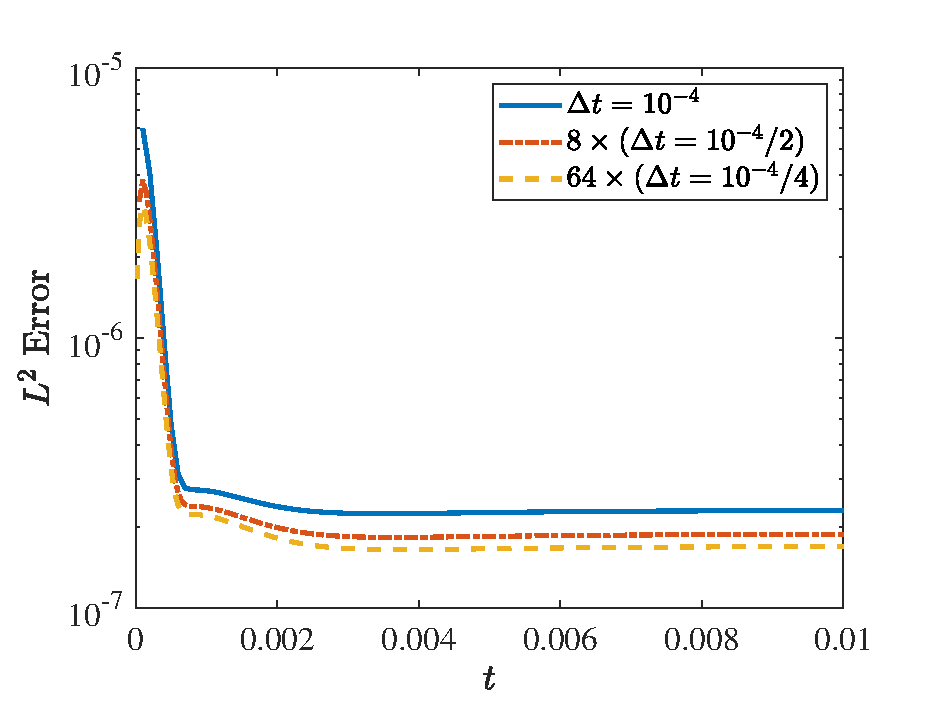
\includegraphics[width=70mm]{Local/RK3N8.eps}}
\subfigure[Forward Euler]{
\label{fig:FEN8}
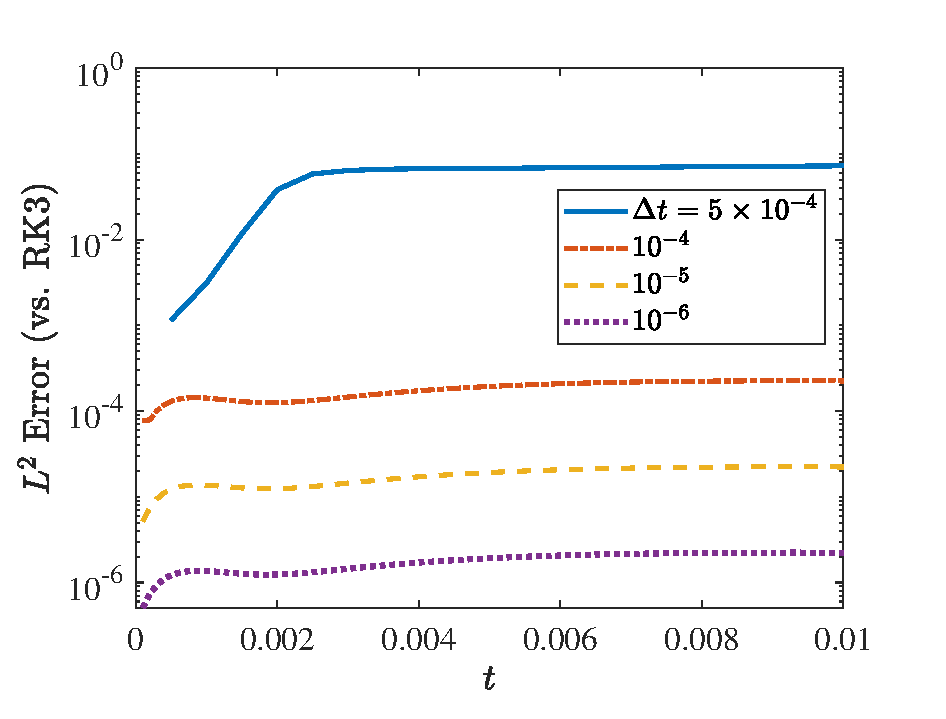
\includegraphics[width=70mm]{Local/FEErrorN8.eps}}
%\subfigure[Our explicit scheme]{
%\label{fig:UsEx}
%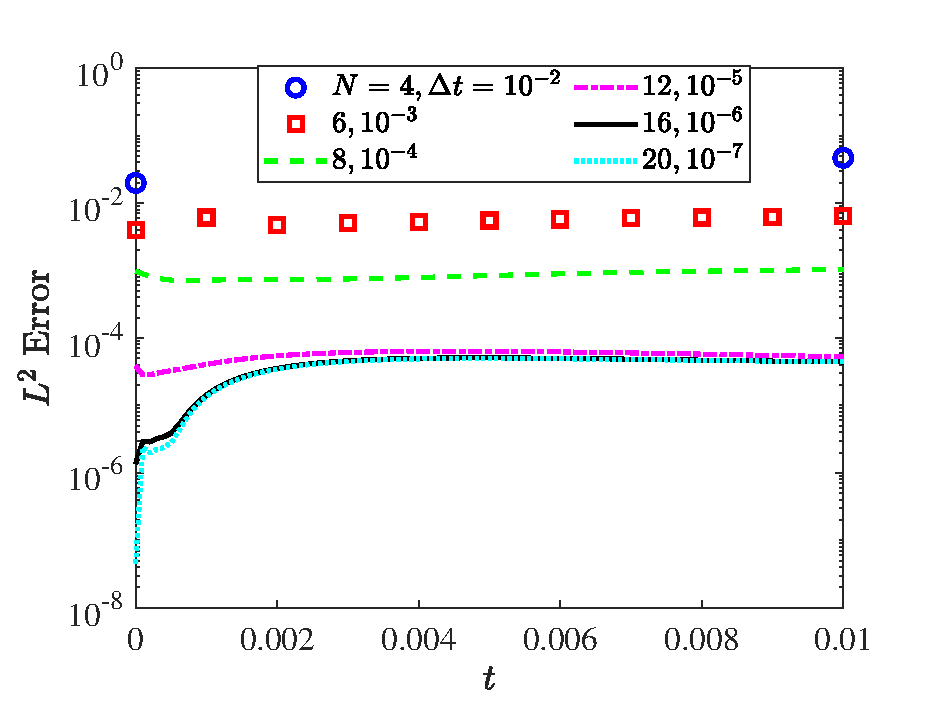
\includegraphics[width=70mm]{Local/UsTemporalSpatial.eps}}
\caption{Temporal accuracy for a fixed spatial discretization $N=8$. (a) $L^2$ error for SSP RK3 on $N=8$ (with respect to successive refinements in $\Delta t$ by a factor of 2). The error for $\Delta t =10^{-4}$ (blue line) is approximately 8 times the error for $\Delta t = 10^{-4}/2$ (dashed/dotted red line) and 64 times the error for $\Delta t =10^{-4}/4$. The scheme is therefore third-order accurate. (b) Accuracy of the forward Euler method when compared to the ``exact solution'' from SSP RK3. $\Delta t = 5 \times 10^{-4}$ (blue line) is clearly inaccurate; it is likely too close to the stability limit. $\Delta t=10^{-4}$ (dashed/dotted red), $\Delta t =10^{-5}$ (dashed yellow), and $\Delta t =10^{-6}$ (dotted purple) demonstrate first order convergence starting at an $L^2$ error of $10^{-4}$. We conclude that the first-order method is sufficient since temporal error is less than spatial error for any $\Delta t \leq 2 \times 10^{-4}$.} 
\end{figure}

\subsubsection{Spatio-temporal accuracy of our scheme}
Since we cannot choose any timestep, we seek some kind of comparison between our method and Floren's. That is, a way to compare to Fig.\ \ref{fig:Flortemp}. We therefore set up the following experiment: consider spatial discretizations from $N=6, 8, \dots 20$. We run the \textit{forward Euler} temporal integrator with \textit{the first stable timestep that is a power of 10}. The accuracy of this temporal integration is verfied by ensuring the maximum $L^2$ error in time is of the same order of magnitude with a $\Delta t$ that is half the relevant power of 10. 

For this section, we return to using Floren's maximally refined evolution as the ``exact'' solution (i.e. the same ``exact'' solution as in Fig.\ \ref{fig:FN12}). 

Shown in Fig.\ \ref{fig:UsEx} is the overall accuracy of our scheme under spatio-temporal refinement. \textbf{In our case, a timestep of $10^{-4}$ is stable up to $N=8$ points, and we get an accuracy of $10^{-3}$. This is an order of magnitude better than Floren, whose errors are spatially dominated for this $\Delta t$. Furthermore, for $\Delta t = 10^{-3}$, (when Floren's spatial and temporal errors are comparable) we still get higher accuracy with $N=6$ than Floren with $\tilde{N}=12$!}



\begin{figure}
\centering 
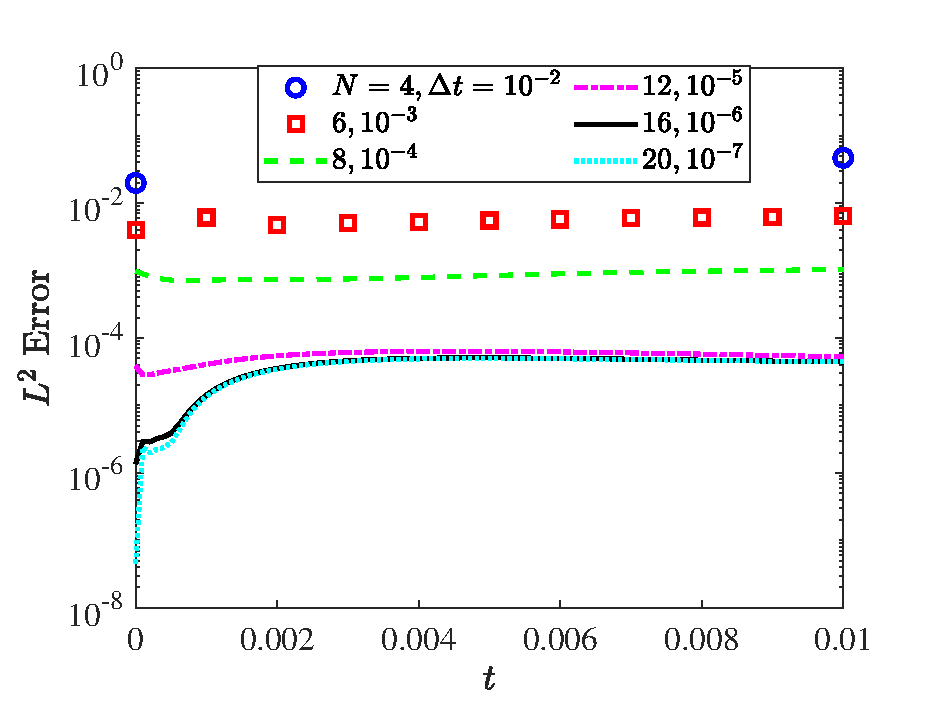
\includegraphics[width=70mm]{Local/UsTemporalSpatial.eps}
\caption{Overall spatio-temporal accuracy of our scheme. Timestep is the first stable power of 10 using forward Euler integration for a given spatial discretization. Recall that the relative error in displacement is approximately 10 times the $L^2$ error. } 
\label{fig:UsEx}
\end{figure}

\subsection{Implicit timestepping}
\subsubsection{Backward Euler}
We recall that we can define $\bm{f}^E = \bm{L}\bm{X}$ on the type 1 grid. With this in mind, we can write the equations for a backward Euler update as
\begin{gather}
\label{eq:tup}
\bm{X}^{n+1} = \bm{X}^{n} + \Delta t  \bm{K} \bm{\alpha} \\[2 pt]
\label{eq:BEeqn}
\bm{K}\bm{\alpha}= \bm{M}^n\left(\bm{\lambda}+\left(\bm{f}^E\right)^{n+1}\right)+\bm{U}_0^{n}\\[2 pt]
\bm{K}^* \bm{\lambda}=\begin{pmatrix} \bm{0}\\[2 pt] -\bm{I}^*\left(\bm{f}^E\right)^{n+1}\end{pmatrix}
\end{gather}
Now suppose that $\bm{U}_0$ is a time-dependent function of $\bm{X}$ (not necessarily linear). Then Eq.\ \eqref{eq:tup} can then be used to rewrite these equations in block form as
\begin{equation}
\label{eq:impsolve}
\bm{A}\bm{y}=
    \begin{pmatrix}
    -\bm{M} &\bm{K}-\Delta t \bm{MLK} \\[4 pt]
   \bm{K}^* &\begin{pmatrix} \bm{0}\\[2 pt]\Delta t \bm{I}^*\bm{LK}\end{pmatrix} 
    \end{pmatrix}^n
    \begin{pmatrix} 
    \bm{\lambda}\\[4 pt]
    \bm{\alpha}\\[4 pt]
    \end{pmatrix} =  \begin{pmatrix} 
   \bm{ML}\bm{X}^n+\bm{U}_0(\bm{X}^n)\\[4 pt]
    \begin{pmatrix} \bm{0}\\[4 pt]
    -\bm{I}^*\bm{L}\bm{X}^n \end{pmatrix}
    \end{pmatrix}. 
\end{equation}

The matrices $\bm{M}$ and $\bm{K}$ depend on $\bm{X}$, and these are treated explicitly. The bending force $\bm{f}^E = \bm{L}\bm{X}$ is always treated implicitly. Note that this results in an $(5N+1)^2$ linear system, which is exactly the same size as in the explicit case, Eq.\ \eqref{eq:saddlept}. 

Now, we saw in Section \ref{sec:space} that the $L^2$ spatial error of our discretization is $\approx 10^{-3}$. However, in Fig.\ \ref{fig:FEN8}, we saw that temporal error near the boundary of the stability region is $10^{-4}$. If we used a larger timestep than $\Delta t = 1-2 \times 10^{4}$, we saw ballooning errors. In this section, we ask whether we can ``fix'' this with implicit timestepping. 

Table \ref{tab:imp} shows the ``savings'' when using backward Euler for different $N$. All of the errors are the maximal $L^2$ error over time. The first column is the spatial error, which is the difference between an RK3 simulation (accurate to 10 digits) of the given $N$ and an RK3 simulation of $N=20$ (which we take as the exact solution). Our goal is for the temporal error, which is the difference between a given ($N$,\, $\Delta t$) pair and the ``exact'' RK3 solution for the same $N$, to be on the same order as the spatial error. Table \ref{tab:imp} shows what timestep is necessary for this.

Considering $N=4$ and $N=8$, we see that the forward Euler method is limited by stability and we can get a savings by switching to backward Euler. For $N > 8$, the spatial discretization is converging so rapidly that we are limited by accuracy; and forward Euler and backward Euler get the same result. So it appears that backward Euler is not particularly advantageous (at least for this very smooth problem), except for $N=8$ when we get a factor of 5. 


%\begin{figure}
%\centering 
%\subfigure[Temporal Errors]{
%\label{fig:tempImp}
%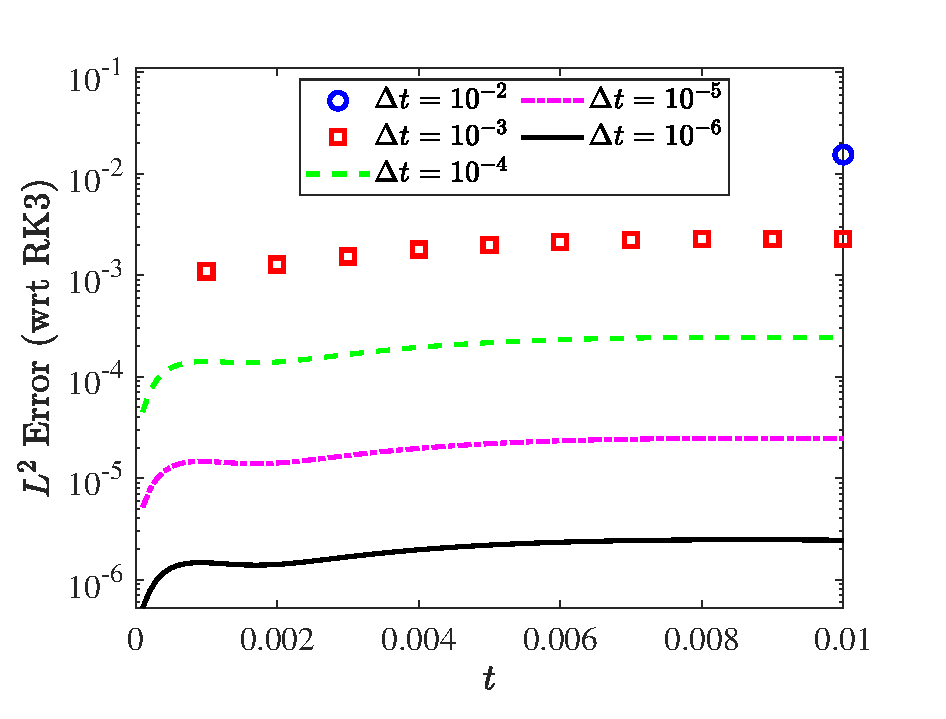
\includegraphics[width=70mm]{Local/ImplicitRK3Er.eps}}
%\subfigure[Spatio-temporal Errors]{
%\label{fig:STImp}
%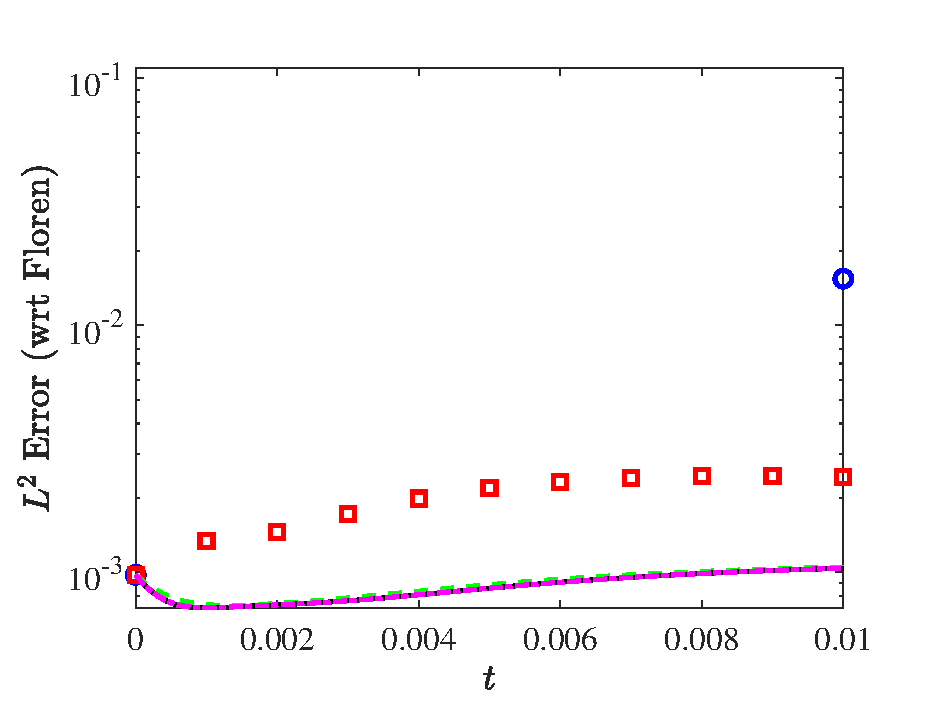
\includegraphics[width=70mm]{Local/ImplicitFlorenEr.eps}}
%\caption{Effect of implicit time-stepping on spatio-temporal error. (a) $L^2$ error over time when comparing with the explicit RK3 solution (known to be accurate to 10 digits). The time integrator is first order, and we can get an $L^2$ error of $\approx 2 \times 10^{-3}$ by taking $\Delta t =10^{-3}$, previously impossible due to stability. Color scheme is the same as Fig. \ref{fig:Flortemp}. (b) Total $L^2$ error using Floren's maximally refined solution as the exact solution. Any timestep $\leq 10^{-4}$ isolates the $10^{-3}$ spatial error. $\Delta t =10^{-3}$ gives an ideal balance of spatial and temporal error.} 
%\end{figure}

\begin{table}
\centering
\begin{tabular}{c|c|c|c|c|c|c|c} 
$N$ & Spatial Er & FE $\Delta t$ &  FE Temp Er & BE $\Delta t$ & BE Temp Er & CN $\Delta t$ & CN Temp Er \\
\hline
4 & 2.23e-2 & $5 \times 10^{-3}$ & 1.35e-2 & $10^{-2}$ & 1.98e-2 &  $10^{-2}$ & 1.28e-2\\[2 pt]
8 & 1.04e-3 & $2 \times 10^{-4}$ & 5.60e-4 & $10^{-3}$ & 2.29e-3 &  $2 \times 10^{-3}$ & 1.58e-3\\[2 pt]
12 & 3.83e-5 & $10^{-5}$ & 2.23e-5&  $10^{-5}$ & 2.47e-5 &  $2 \times 10^{-4}$ & 2.69e-5\\[2 pt]
16 & 2.32e-6 &  $10^{-6}$ & 2.23e-6& $10^{-6}$ & 2.48e-6 &  $5 \times 10^{-5}$ & 1.72e-6
\end{tabular}
\caption{Comparing the required timestep to match the spatial error (measured against $N=20$ RK3) with the temporal error (measured against the RK3 spatial solution for that $N$) using  forward Euler (FE), backward Euler (BE), and Crank-Nicolson (CN). All errors are maximum $L^2$ errors over time. }
\label{tab:imp}
\end{table}

\subsubsection{Crank-Nicolson}
We combine Crank-Nicolson with a linear multi-step method to obtain a second-order scheme with one solver per timestep. Specifically, we set
\begin{equation}
\label{eq:LMM}
\bm{X}^{n+1/2, *} = \frac{3}{2}\bm{X}^n - \frac{1}{2}\bm{X}^{n-1}.
\end{equation}
We then solve 
\begin{equation}
\label{eq:CNsolve}
\bm{A}\bm{y}=
    \begin{pmatrix}
    -\bm{M} &\bm{K}-\frac{1}{2}\Delta t \bm{MLK}\\[4 pt]
   \bm{K}^* &\begin{pmatrix} \bm{0}\\[2 pt]\frac{1}{2}\Delta t \bm{I}^*\bm{LK}\end{pmatrix} 
    \end{pmatrix}^{n+1/2, *}
    \begin{pmatrix} 
    \bm{\lambda}\\[4 pt]
    \bm{\alpha}\\[4 pt]
    \end{pmatrix} =  \begin{pmatrix} 
   \bm{ML}\bm{X}^n+\bm{U}_0(\bm{X}^{n+1/2, *})\\[4 pt]
    \begin{pmatrix} \bm{0}\\[4 pt]
    -\bm{I}^*\bm{L}\bm{X}^n \end{pmatrix}
    \end{pmatrix}.
\end{equation}
Eq.\ \eqref{eq:CNsolve} is now the system to be solved at every timestep, with the operators $\bm{M}$ and $\bm{K}$ evaluated using Eq.\ \eqref{eq:LMM}. One we have computed $\V{\alpha}$, we use a discrete form of Eq.\ \eqref{eq:Xsupdate} to update the tangent vectors. Our goal is to rotate $\V{X}_s^n$ on the unit sphere by the vector $\V{\Omega}^{n+1/2} =  \V{\Omega}\left(\V{X}^{n+1/2,*},\V{\alpha}^{n+1/2}\right)$. Using the Rodrigues rotation formula with $\Omega = \norm{\V{\Omega}}$, we compute the rotated $\V{X}_s$ as
\begin{equation}
\V{X}_s^{n+1} = \V{X}_s^n \cos{\left(\Omega^{n+1/2}\D t\right)} + \left(\hat{\V{\Omega}}^{n+1/2} \times \V{X}_s^n \right)  \sin{\left(\Omega^{n+1/2}\D t\right)}+\hat{\V{\Omega}}^{n+1/2}\left(\hat{\V{\Omega}}^{n+1/2} \cdot \V{X}_s^n\right)\left(1-\cos{\left(\Omega^{n+1/2}\D t\right)}\right).
\end{equation}
We then compute $\V{X}^{n+1}$ via Chebyshev integration. Note that now $\displaystyle{\frac{\V{X}^{n+1}-\V{X}^n}{\Delta t} = \M{K}\V{\alpha}}$ is true to second order in $\Delta t$, rather than exactly. 

Because we saw that backward Euler gave little to no savings over forward Euler, our goal in this section is to determine whether a \textit{second-order} implicit scheme (which requires one solve per timestep) gives a savings over an explicit one. 
 
Fig.\ \ref{fig:FECN} shows that the Crank-Nicolson scheme is second-order accurate and gives a much lower temporal error for $\Delta t \leq 10^{-3}$ than backward Euler for $N=8$. Furthermore, we see in Table \ref{tab:imp} that the Crank-Nicolson temporal update can give a temporal error comparable to the spatial error for much larger timesteps than forward/backward Euler. In particular, for $N=4, 8, 12$, and 16, we see a savings from Crank-Nicolson (over forward Euler) that is a factor of 1, 10, 20, and 50. This comes at no extra cost (other than a possibly dangerous extrapolation step), since we are doing a $(5N+1)^2$ least squares solve once per timestep in all cases. 

\begin{figure}
\centering 
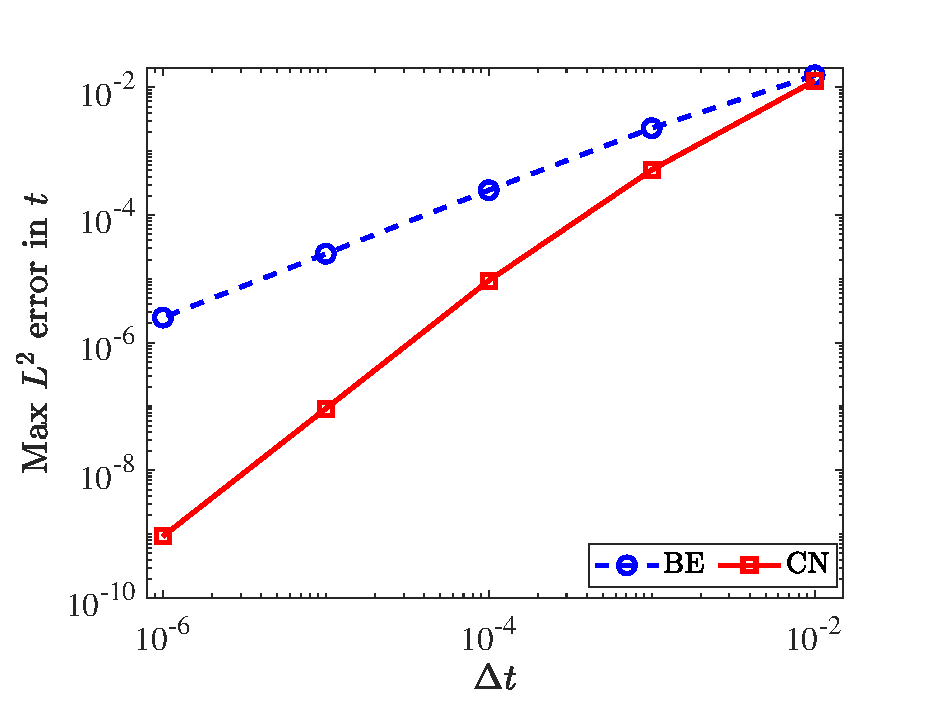
\includegraphics[width=70mm]{Local/FECN.eps}
\caption{Comparing the temporal error from backward Euler (red circles) and Crank-Nicolson (blue squares) for $N=8$. Shown is the maximum $L^2$ error (wrt the RK3 explicit solution accurate to 10 digits) over time for different $\Delta t$. First order convergence is observed for backward Euler, and second-order convergence is observed for Crank-Nicolson. Table \ref{tab:imp} has more details on the savings that can be obtained for different $N$.  } 
\label{fig:FECN}
\end{figure}

\bibliographystyle{plain}

\bibliography{SlenderBib}

\end{document}
